\documentclass[a4paper,12pt]{article}
\parindent 0pt
\parskip 1mm
\usepackage{amsmath}
\usepackage[dvips]{epsfig}

\begin{document}
\begin{center}

{\Large\bf MA 555 - Numerical Analysis}
\bigskip

{\large\bf Homework \# 1}
\smallskip

{\large\bf John Joseph}
\end{center}

\bigskip
{\bf 1. Minimize $I(a,b)=\int_{-1}^1(x^2+ax+b)^2 dx $. Graph the function and locate its maximum value over the interval [-1,1].  }

In order to minimize this function we take the partial derivatives of $I$ with respect to $a$ and $b$ and set them equal to 0. We end up with a linear system with two equations and two unknowns. Starting with $a$...

\begin{equation}
\frac{\partial I}{\partial a} = 2 \int_{-1}^1(x^2+ax+b)(x) dx = 0
\end{equation}

By solving this integral in Mathematica we get the result 

\begin{equation}
0 = \frac{-2a}{3}
\end{equation}

and conclude that $a=0$. Now to $b$...

\begin{equation}
\frac{\partial I}{\partial b} = 2 \int_{-1}^1(x^2+ax+b) dx = 0
\end{equation}

Again solving in Mathematica we see that

\begin{equation}
0 = \frac{2}{3} + 2b
\end{equation}

\begin{equation}
b = -\frac{1}{3}
\end{equation}

Therefore, our minimized function is 

\begin{equation}
I_{min}(a,b) = \int_{-1}^1(x^2-\frac{1}{3})^2 dx
\end{equation}

\vfil\eject

Graphing the quadratic function $x^2-\frac{1}{3}$ yields the following figure

\begin{center}
  \begin{figure}[h!]
    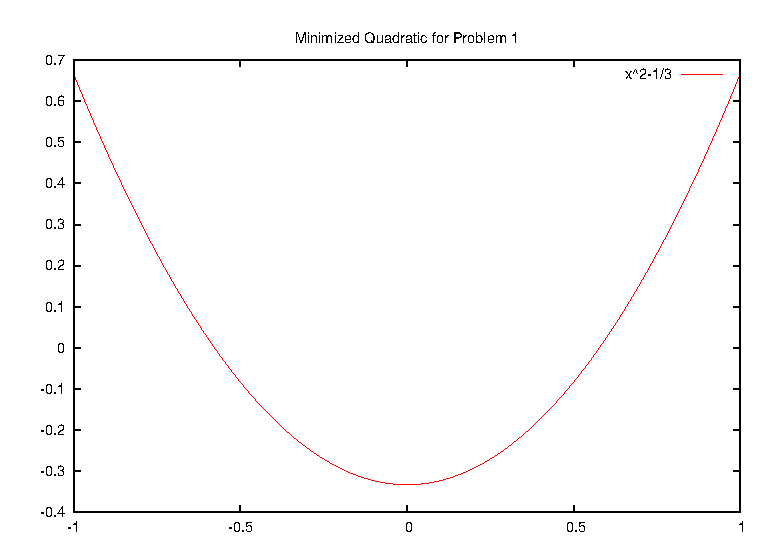
\epsfig{file=prob1,width=13cm,height=8cm}
  \end{figure}
\end{center}


from which it is clear that the maximum value is $\frac{2}{3}$, occuring at $|x|=1$.

\vspace{2mm}

{\bf 2. Minimize a similar function $I(c,d)$ using the previous result as a weight function. }

\begin{equation}
\frac{\partial I}{\partial c} = 2 \int_{-1}^1(x^2-\frac{1}{3})^2(x^2+cx+d)(x) dx = 0
\end{equation}

Solving this integral in Mathematica gives the result

\begin{equation}
0 = \frac{88c}{945}
\end{equation}

From which we conclude $c=0$. Moving on to d...

\begin{equation}
\frac{\partial I}{\partial d} = 2 \int_{-1}^1(x^2-\frac{1}{3})^2(x^2+cx+d) dx = 0
\end{equation}

Solving this integral in Mathematica gives the result

\begin{equation}
0 = \frac{44}{945}+\frac{84d}{945}
\end{equation}

Solving for $d$ shows that $d=-\frac{11}{21}$. Intuition (and Professor Fried) tells us that the best value we can get is $-frac{1}{2}$, so this is pretty good. Graphing the quadratic function $x^2-\frac{11}{21}$ yeilds the figure

\begin{center}
  \begin{figure}[h!]
    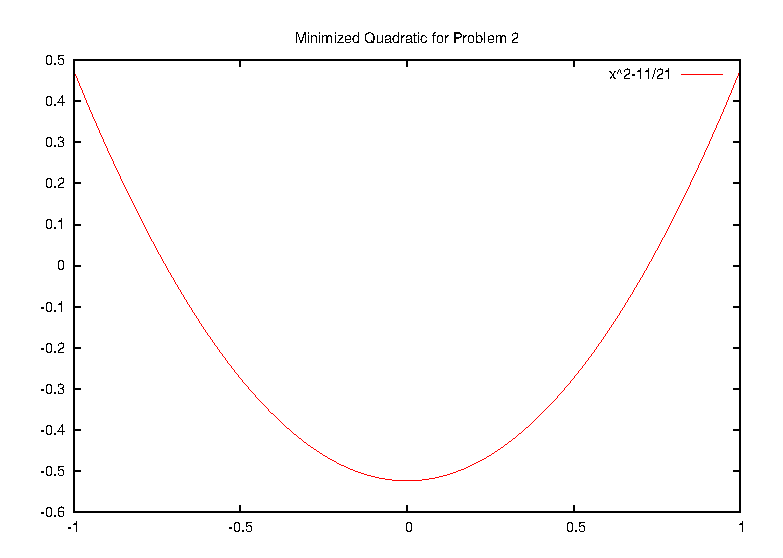
\epsfig{file=prob2,width=13cm,height=8cm}
  \end{figure}
\end{center}

The max clearly occurs at $|x|=1$, and solving the equation for $x=\pm 1$ yeilds tha max of $\frac{10}{21}$.

\vspace{2mm}

{\bf 3. Minimize the function $I(b)=\int_{-1}^1(x^3-bx)^2 dx$.} 

\begin{equation}
\frac{\partial I}{\partial b} = 2 \int_{-1}^1(x^3-bx)(x) dx = 0
\end{equation}

Solving this integral yields

\begin{equation}
0 = \frac{2}{5}-\frac{2b}{3}
\end{equation}

From which we see that $b=\frac{3}{5}$ and 

\begin{equation}
I_{min}(b)=\int_{-1}^1(x^3-\frac{3}{5})^2 dx
\end{equation}

\vfil\eject

\vspace{2mm}

{\bf 4. Calculate $x=\frac{1.23678-1.23456}{1.23555-1.23444}$ using 4,5, and 6 digit arithmetic.}

Here is a copy and paste from my terminal. I used Python and its round function.

\begin{verbatim}
>>> for n in range (4,7):
...     x=round(1.23678-1.23456,n)/round(1.23555-1.23444,n)
...     print str(x) + ", " + str(n)
... 
2.0, 4
2.0, 5
2.0, 6
\end{verbatim}

This seemed strange at first, but it makes sense if you actually do it out by hand. The $4^{th}$, $5^{th}$, and $6^{th}$ always have the same difference during subtraction. 


\end{document}
